\subsection{Characterizing Loss Spikes}
\label{subsec:characterization}

\begin{figure*}[!t]
\centering
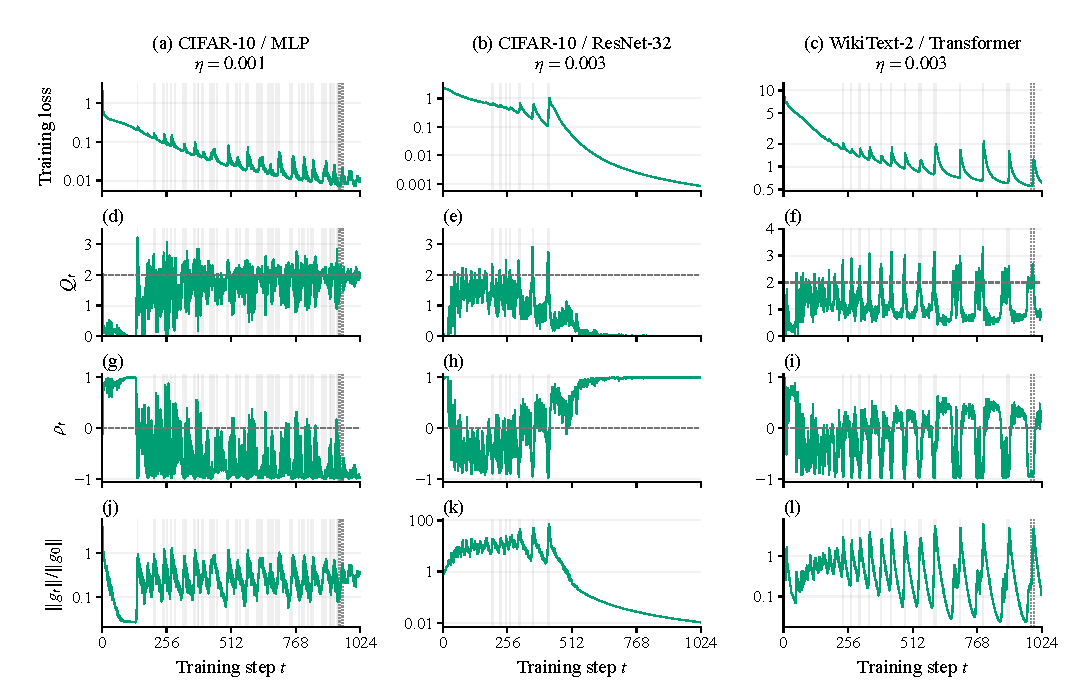
\includegraphics[width=\textwidth]{figures/00-high-lr-overview-cifar10-mlp-resnet-wikitext2-transformer.pdf}
\caption{Loss spikes and consecutive-gradient behavior under full-objective Adam. Columns are MLP, ResNet-32, and Transformer, at learning rates $.001/.003/.003$, with one initialization per model. Rows show loss, the gradient-projected response $\eta\widehat\kappa_t$, consecutive-gradient cosine, and gradient norm relative to initialization. Filled gray bands mark the rising portions of recovered loss excursions exceeding 10\%; outlined bands mark excursions whose recovery is not observed. Events are selected from loss alone. Training step $t$ counts completed updates; gradient measurements are made at $\theta_t$, before the next update. Loss is recorded through 1,024 updates and gradients through 1,023. The $\eta\widehat\kappa_t$ axis starts at zero; negative values lie outside its displayed range.}
\label{fig:adam-overview}
\end{figure*}

Unlike the sustained GD oscillations, the Adam trajectories exhibit
distinct excursions and recoveries. This is consistent with the adaptive
preconditioner mechanism analyzed by Bai et al.~\cite{bai2026spikes}:
changing second moments can alter the effective step size independently
of changes in the underlying Hessian. Our measurements describe how the
resulting motion appears in consecutive gradients. Early constructive
intervals give way to persistent reversal.
Prominent excursions occur with negative cosine and growing gradient
norms, producing large peaks in $\eta\widehat\kappa_t$. In ResNet and
Transformer, recovery often includes renewed constructive alignment and
falling norms.

The loss can reach lower values after an excursion. Such an excursion
could accompany movement into another basin, while momentum can delay
the update's response to a newly changing gradient direction. Whether
that movement helps depends on the current landscape, architecture,
and optimizer state. Related work on SGD catapults shows that spikes can
accompany improved feature learning~\cite{zhu2024catapults}; their role
under Adam must likewise be evaluated together with subsequent progress.

After computing the raw gradient, but before applying the next update,
we may want to classify whether that update will increase the loss.
Let $L_t=\mathcal L(\theta_t)$ and define an increase as
$(L_{t+1}-L_t)/L_t\geq0.001$. At decision step $t$, both $g_t$ and $L_t$
are available. However, the pair $(g_{t-1},g_t)$ describes the response
to the preceding update, from $\theta_{t-1}$ to $\theta_t$. Using it to
classify the outgoing update tests whether that response carries forward.
For quadratic full-batch plain GD, the strict condition
$\eta\widehat\kappa_t>2$ exactly characterizes a positive loss change
on the preceding step. This exact retrospective equivalence does not
extend to a finite nonlinear step or to Adam, whose applied direction
also depends on its moments.

Table~\ref{tab:severity} compares the gradient conditions with the
simple history rule $L_t>L_{t-1}$. Accuracy is the fraction of all
decisions classified correctly. Warning hit rate is the fraction of
warnings followed by an increase; lift divides this rate by the overall
frequency of increases. Together they distinguish correct classification
from how informative an issued warning is.

\begin{table*}[!t]
\centering\small
\caption{Before-update diagnostics for a next-step loss increase of at least 0.1\%. All 1,023 decisions per model are retained. Acc. is classification accuracy, $(\mathrm{TP}+\mathrm{TN})/1023$; Hit is the percentage of warnings followed by the target (precision); lift is Hit divided by the baseline event rate. The no-increase baseline exposes class imbalance. The last two conditions agree on these data and are two forms of the same diagnostic.}
\label{tab:severity}
\setlength{\tabcolsep}{4pt}
\begin{tabular}{@{}lrrrrrrrrr@{}}
\toprule
& \multicolumn{3}{c}{MLP} & \multicolumn{3}{c}{ResNet} & \multicolumn{3}{c}{Transformer} \\
Condition & Acc. (\%) & Hit (\%) & Lift ($\times$) & Acc. (\%) & Hit (\%) & Lift ($\times$) & Acc. (\%) & Hit (\%) & Lift ($\times$) \\
\midrule
Baseline event rate & \multicolumn{3}{c}{446/1023 (43.6\%)} & \multicolumn{3}{c}{88/1023 (8.6\%)} & \multicolumn{3}{c}{142/1023 (13.9\%)} \\
\midrule
Always predict no increase & 56.4 & -- & -- & 91.4 & -- & -- & 86.1 & -- & -- \\
Always predict increase & 43.6 & 43.6 & 1.00 & 8.6 & 8.6 & 1.00 & 13.9 & 13.9 & 1.00 \\
$L_t>L_{t-1}$ & 58.1 & 51.9 & 1.19 & 89.0 & 36.8 & 4.28 & 86.5 & 51.3 & 3.70 \\
$\rho_t<0$ & 54.4 & 48.8 & 1.12 & 77.9 & 27.0 & 3.14 & 61.6 & 25.9 & 1.87 \\
$\|g_t\|>\|g_{t-1}\|$ & 53.5 & 47.3 & 1.08 & 68.7 & 14.2 & 1.65 & 63.1 & 22.1 & 1.59 \\
$\rho_t<-\|g_{t-1}\|/\|g_t\|$ & 59.9 & 55.8 & 1.28 & 92.0 & 58.3 & 6.78 & 87.2 & 53.7 & 3.87 \\
$\eta\widehat\kappa_t\geq2$ & 59.9 & 55.8 & 1.28 & 92.0 & 58.3 & 6.78 & 87.2 & 53.7 & 3.87 \\
\bottomrule
\end{tabular}
\end{table*}


The \emph{destructive loss-spike condition} combines reversal with
sufficient gradient growth, $\rho_t<0$ and
$\|g_t\|/\|g_{t-1}\|>-1/\rho_t$. It gives higher accuracy and warning
lift than the previous-loss-rise rule in all three cases. Reversal or
norm growth alone is less selective. The angle/norm condition is
algebraically equivalent to $\eta\widehat\kappa_t>2$; their identical
table entries verify the two implementations, rather than constitute
independent evidence. The non-strict threshold gives the same flags
here because no observed value equals two. The warning lifts are
$1.28\times$, $6.78\times$, and $3.87\times$ for MLP, ResNet, and
Transformer. These signals contain information before the next update,
although the gains in overall accuracy over always predicting no
increase are modest.

A loss curve and a whole-network gradient still leave an important
question unanswered: what is changing inside the network during these
oscillations? We next examine that functional expression directly.
